\documentclass[conference]{IEEEtran}
\IEEEoverridecommandlockouts

\usepackage[utf8]{inputenc}
\usepackage[T1]{fontenc}
\usepackage{cite}
\usepackage{amsmath,amssymb}
\usepackage{graphicx}
\usepackage{booktabs}
\usepackage{hyperref}
\usepackage{xcolor}

\usepackage{ieeeextras}

\graphicspath{{figuras/}{../docs/images/}}

\hypersetup{colorlinks=true,linkcolor=blue,citecolor=blue,urlcolor=blue}

\begin{document}

\title{Ingressos distribu\'idos: algoritmos cl\'assicos em cluster Docker}

\author{
\IEEEauthorblockN{Lucas F\'elix}
\IEEEauthorblockA{RA: 247064\\
Instituto de Computação -- UNICAMP}
\and
\IEEEauthorblockN{Renilson Concei\c{c}\~ao de Luna Junior}
\IEEEauthorblockA{RA: 247358\\
Instituto de Computação -- UNICAMP}
}

\maketitle

\begin{abstract}
Implementamos e avaliamos um sistema de venda de ingressos com quatro
mecanismos distribuídos: relógio lógico de Lamport para ordem total de
eventos, exclusão mútua de Ricart-Agrawala, compromisso atômico em duas
fases (2PC) e detector de falhas por \emph{heartbeat}. A solução roda em
contêineres Docker (API FastAPI, três \emph{helpers} e PostgreSQL
primário com três réplicas) e expõe cenários de correção via testes
automatizados e ensaios de carga HTTP com variação de concorrência.
\end{abstract}

\begin{IEEEkeywords}
sistemas distribuídos, Lamport, Ricart-Agrawala, two-phase commit, heartbeat
\end{IEEEkeywords}

\section*{Informações de entrega}
\textbf{Repositório:} \pendente{URL do GitLab da disciplina}\\
\textbf{Vídeo:} \pendente{URL do vídeo de demonstração ($\sim$5\,min)}

\section{Introdução}

O Trabalho~2 de MC714 exige implementar algoritmos distribuídos
complementares, explicitar o modelo de sistema e medir o comportamento
sob carga e falhas~\cite{vanSteen2023}. Adotamos o domínio de
\textbf{ingressos}: eventos de negócio devem ser ordenados
causalmente, compras concorrentes não podem corromper estoque, transações
de compra devem ser atômicas entre participantes e nós auxiliares precisam
ser monitorados.

Implementamos \emph{quatro} algoritmos (dois obrigatórios e dois de
bônus): (i)~Lamport; (ii)~Ricart-Agrawala; (iii)~2PC; (iv)~detector por
\emph{heartbeat}. Todos são orquestrados pela API em
\texttt{server/app/main.py} e comunicam-se por HTTP/JSON entre contêineres.

\section{Modelo do sistema}

Tabela~\ref{tab:modelo} resume hipóteses comuns. O tempo é
\textbf{parcialmente síncrono}: mensagens não têm limite superior de
atraso, mas aplicações usam \emph{timeouts} explícitos (3--5\,s) em chamadas
RPC. Canais são TCP ordenados, ponto a ponto, sem duplicação em condições
normais. Falhas consideradas são \textbf{crash-stop} e
\textbf{crash-recovery} em nós lógicos; não há tolerância bizantina.
Contêineres em um único host representam domínios de falha distintos apenas
de forma lógica---limitação discutida na Seção~\ref{sec:limitacoes}.

\begin{table}[!t]
\centering
\caption{Propriedades de correção por algoritmo.}
\label{tab:modelo}
\scriptsize
\begin{tabular}{@{}p{0.24\columnwidth}p{0.68\columnwidth}@{}}
\toprule
Algoritmo & Segurança / vivacidade \\
\midrule
Lamport & Ordem total consistente com relação \emph{happens-before}; tupla $(c, id)$ desempata. \\
Ricart-Agrawala & No máximo um nó em seção crítica; solicitações eventualmente entram se não houver falha permanente. \\
2PC & Atomicidade: todos \emph{commit} ou todos \emph{abort}; log durável no primário. \\
Heartbeat & Eventual detecção após $\geq \texttt{max\_missed}$ pings falhos. \\
\bottomrule
\end{tabular}
\end{table}

\section{Arquitetura}

A Fig.~\ref{fig:arquitetura} mostra o \emph{cluster}: coordenador
FastAPI (\texttt{api-coordinator}), três \texttt{helper-node-*}
(participantes dos protocolos) e PostgreSQL com \textbf{um primário e três
réplicas} em \emph{streaming replication}. O primário persiste eventos
ordenados, compras e o log \texttt{two\_phase\_transactions}.

\begin{figure}[!t]
\centering
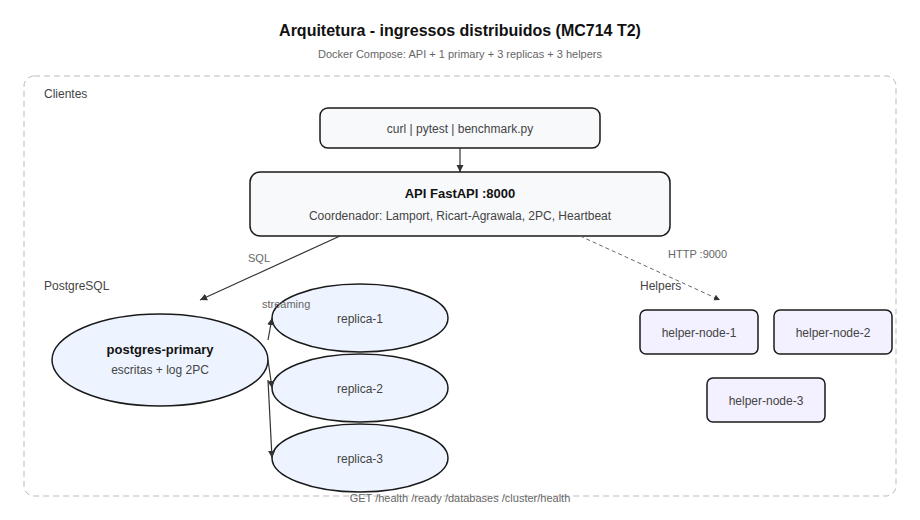
\includegraphics[width=\linewidth]{arquitetura-cluster.png}
\caption{Topologia lógica do sistema (API, helpers e banco).}
\label{fig:arquitetura}
\end{figure}

\section{Comunicação}

Usamos HTTP/1.1 com corpo JSON entre contêineres na rede \texttt{mc714-net}.
Chamadas do coordenador aos helpers definem \texttt{timeout} de 3\,s
(2PC) ou 5\,s (mutex). Semantics: \emph{at-most-once} por requisição, sem
retransmissão automática; falhas de rede manifestam-se como \texttt{504} ou
voto \texttt{NO} no 2PC. Redis ou brokers não foram usados, evitando
coordenação opaca externa.

\section{Algoritmos e correção}

\textbf{Lamport} --- \texttt{POST/GET /events/ordered}: cada evento recebe
timestamp $(clock, node\_id)$; gravação no primário e propagação assíncrona
do relógio aos helpers. A leitura ordena por \texttt{lamport\_clock ASC,
node\_id ASC}.

\textbf{Ricart-Agrawala} --- \texttt{POST /tickets/buy-mutex}: o
coordenador envia \texttt{REQUEST} a todos os helpers, aguarda \texttt{REPLY}
e executa a seção crítica (atualização de estoque com \texttt{FOR UPDATE}).

\textbf{2PC} --- \texttt{POST /tickets/buy-2pc}: fase \texttt{PREPARE}
com votação unânime; \texttt{COMMIT} ou \texttt{ABORT} na fase~2; estado
persistido no primário. Compras com quantidade $> 50$ são rejeitadas na
validação do modelo (cenário de \emph{abort}).

\textbf{Heartbeat} --- \texttt{GET /cluster/health}: laço assíncrono com
intervalo de 2\,s, \texttt{max\_missed}=3 e \emph{timeout} de 1{,}5\,s por
ping. Falha de helper é injetada com \texttt{docker compose stop}.

Testes: 15 casos em \texttt{tests/unit} e \texttt{tests/integration}
(causalidade Lamport, exclusão mútua simulada entre dois nós, votos 2PC,
contagem de \emph{missed} do detector e \emph{ticks} concorrentes no relógio).
Cenários de falha incluem: (i)~abort 2PC com quantidade acima do limite;
(ii)~simulação de pings falhos at\'e \texttt{max\_missed}; (iii)~timeout de
mutex sob contenção. A su\'ite roda com \texttt{pytest} sem Docker nos testes
unit\'arios.

\section{Replicação de dados}

O PostgreSQL primário replica WAL para tr\^es \emph{standbys}. O log
\texttt{two\_phase\_transactions} garante auditabilidade do coordenador 2PC.
Eventos Lamport residem em \texttt{distributed\_ordered\_events}. Esta camada
não implementa quórum de escrita; participantes lógicos do 2PC são os
\texttt{helpers}, não as réplicas.

\section{Avaliação experimental}
\label{sec:exp}

\begin{table}[!t]
\centering
\caption{Configuração do ambiente experimental.}
\label{tab:ambiente}
\scriptsize
\begin{tabular}{@{}p{0.22\columnwidth}p{0.68\columnwidth}@{}}
\toprule
Item & Valor \\
\midrule
CPU & Intel(R) Core(TM) i5-7200U CPU @ 2.50GHz \\
RAM & 7.1Gi \\
Sistema operacional & Linux 7.0.0-43-generic \#43-Ubuntu SMP PREEMPT\_DYNAMIC Fri Oct 23 13:25:25 UTC 2026 x86\_64 \\
Docker Engine & 29.9.2 \\
Python (benchmark) & Python 3.14.4 \\
PostgreSQL (imagem) & \texttt{postgres:16} \\
Requisições por nível de concorrência & 50 \\
Níveis de concorrência & 1, 5, 10, 20 threads \\
Repetições independentes & 3 (\texttt{run1--3.csv}) \\
Aquecimento & 10 requisições descartadas por nível (pré-ensaio manual) \\
\bottomrule
\end{tabular}
\end{table}


\textbf{Metodologia.} O script \texttt{scripts/benchmark.py} dispara
requisições HTTP concorrentes (1, 5, 10 e 20 \emph{threads}) com 50
repetições por nível. Métricas: taxa de sucesso, vazão (req/s) e latências
média, $p_{50}$, $p_{95}$ e $p_{99}$. O estoque de ingressos é restaurado
antes dos ensaios; executamos três repetições
(\texttt{results/run\{1,2,3\}.csv}).

\textbf{Desempenho sob carga.} Tabela~\ref{tab:experiments} resume o ensaio
em \texttt{results/experiments.csv} (média das três repetições quando
\texttt{experiments\_summary.tex} estiver presente). Regenerar com
\texttt{./scripts/run\_experiments.sh} após \texttt{docker compose up -d}.
Espera-se crescimento de latência em Ricart-Agrawala e 2PC com a
concorrência, pois cada operação exige $O(n)$ mensagens com $n=3$ helpers.
Se a taxa de sucesso estiver abaixo de 100\%, verifique estoque de
ingressos e sa\'ude da API. Na Tabela~\ref{tab:experiments}, lat\^encias
refletem tempos de resposta HTTP mesmo em falhas (ex.: API ou banco
indispon\'iveis durante coleta antiga); ap\'os regenerar o CSV com cluster
ativo, a taxa de sucesso de Lamport tende a 100\% e mutex/2PC dependem do
estoque (semeado com 10\,000 ingressos).

\textbf{An\'alise.} Ricart-Agrawala com 20 \emph{threads} exibe cauda pesada
($p_{95}\approx 5$\,s), consistente com fila de se\c{c}\~ao cr\'itica e
timeouts. Lamport tem menor custo por requisi\c{c}\~ao (uma escrita no
prim\'ario). O 2PC adiciona duas rodadas de mensagens aos tr\^es
participantes, elevando $p_{50}$ de forma moderada sob concorr\^encia
moderada.

\IfFileExists{dados/experiments_summary.tex}{
  \begin{table}[!t]
\centering
\caption{Desempenho por algoritmo e concorrência (cliente HTTP multithread).}
\label{tab:experiments}
\scriptsize
\setlength{\tabcolsep}{3pt}
\begin{tabular}{@{}l r r r r r r@{}}
\toprule
Algoritmo & $T$ & Sucesso (\%) & Vazão & $p_{50}$ & $p_{95}$ & $p_{99}$ \\
 & (threads) &  & (req/s) & (ms) & (ms) & (ms) \\
\midrule
Lamport Ordering & 1 & 100,00 & 115,8 & 8,25 & 11,21 & 14,76 \\
Lamport Ordering & 5 & 100,00 & 114,0 & 37,54 & 107,91 & 122,11 \\
Lamport Ordering & 10 & 100,00 & 100,5 & 104,28 & 141,94 & 164,19 \\
Lamport Ordering & 20 & 100,00 & 119,4 & 147,46 & 164,07 & 174,01 \\
Ricart-Agrawala Mutex & 1 & 100,00 & 79,2 & 10,94 & 20,92 & 53,99 \\
Ricart-Agrawala Mutex & 5 & 96,00 & 9,1 & 51,67 & 1726,66 & 5006,37 \\
Ricart-Agrawala Mutex & 10 & 95,33 & 9,0 & 107,38 & 1823,13 & 5006,50 \\
Ricart-Agrawala Mutex & 20 & 94,00 & 33,7 & 257,50 & 3461,30 & 3501,10 \\
Two-Phase Commit (2PC) & 1 & 100,00 & 48,9 & 19,39 & 27,61 & 46,67 \\
Two-Phase Commit (2PC) & 5 & 100,00 & 56,8 & 85,69 & 125,79 & 131,66 \\
Two-Phase Commit (2PC) & 10 & 100,00 & 63,7 & 147,24 & 212,82 & 230,60 \\
Two-Phase Commit (2PC) & 20 & 100,00 & 61,3 & 295,97 & 488,37 & 563,94 \\
\bottomrule
\end{tabular}
\end{table}

}{
  \begin{table}[!t]
\centering
\caption{Desempenho por algoritmo e concorrência (cliente HTTP multithread).}
\label{tab:experiments}
\scriptsize
\setlength{\tabcolsep}{3pt}
\begin{tabular}{@{}l r r r r r r@{}}
\toprule
Algoritmo & $T$ & Sucesso (\%) & Vazão & $p_{50}$ & $p_{95}$ & $p_{99}$ \\
 & (threads) &  & (req/s) & (ms) & (ms) & (ms) \\
\midrule
Lamport Ordering & 1 & 0,00 & 316,0 & 2,58 & 4,04 & 31,36 \\
Lamport Ordering & 5 & 0,00 & 250,2 & 9,45 & 110,98 & 114,74 \\
Lamport Ordering & 10 & 0,00 & 272,1 & 34,97 & 49,37 & 54,23 \\
Lamport Ordering & 20 & 0,00 & 449,6 & 40,39 & 43,88 & 44,27 \\
Ricart-Agrawala Mutex & 1 & 20,00 & 171,0 & 5,00 & 9,76 & 17,25 \\
Ricart-Agrawala Mutex & 5 & 0,00 & 289,1 & 16,99 & 22,91 & 25,48 \\
Ricart-Agrawala Mutex & 10 & 0,00 & 218,2 & 42,93 & 64,21 & 65,25 \\
Ricart-Agrawala Mutex & 20 & 0,00 & 9,6 & 102,74 & 5005,48 & 5006,08 \\
Two-Phase Commit (2PC) & 1 & 0,00 & 299,6 & 3,18 & 4,67 & 4,85 \\
Two-Phase Commit (2PC) & 5 & 0,00 & 368,8 & 12,94 & 15,52 & 16,86 \\
Two-Phase Commit (2PC) & 10 & 0,00 & 504,0 & 18,48 & 20,84 & 21,02 \\
Two-Phase Commit (2PC) & 20 & 0,00 & 367,2 & 51,70 & 65,61 & 68,19 \\
\bottomrule
\end{tabular}
\end{table}

}

\begin{figure}[!t]
\centering
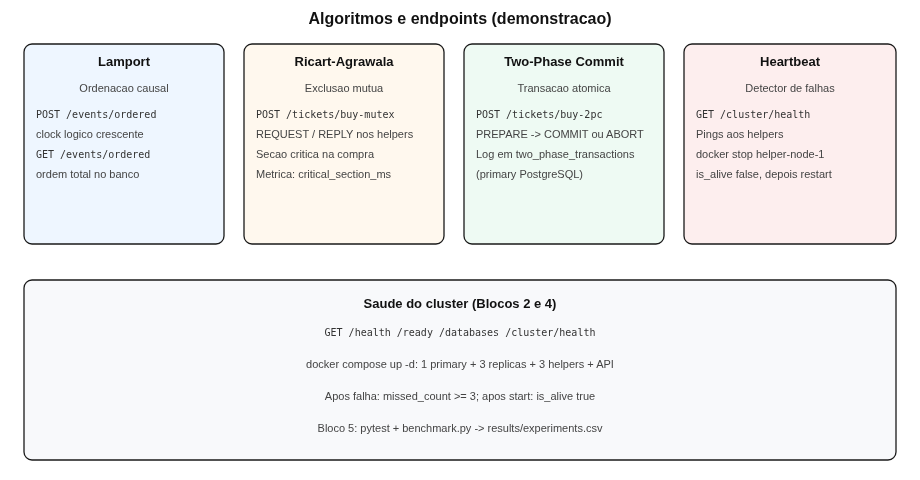
\includegraphics[width=\linewidth]{algoritmos-fluxos.png}
\caption{Fluxos HTTP dos quatro algoritmos.}
\label{fig:fluxos}
\end{figure}

\textbf{Falha e recuperação.} A Tabela~\ref{tab:heartbeat} reporta tempos
do detector. Em produção, a detecção ocorre após três pings falhos em
rodadas espaçadas de 2\,s ($\sim$6--8\,s observados no roteiro de vídeo).

\begin{table}[!t]
\centering
\caption{Tempos do detector de falhas (ensaio com \texttt{interval}=2.0s, \texttt{max\_missed}=3).}
\label{tab:heartbeat}
\begin{tabular}{@{}l r@{}}
\toprule
Métrica & Valor (s) \\
\midrule
Tempo até \texttt{is\_alive=false} após parada simulada & 5.95 \\
Tempo até \texttt{is\_alive=true} após retorno do ping & 2.00 \\
Intervalo configurado entre pings & 2{,}0 \\
Pings perdidos tolerados (\texttt{max\_missed}) & 3 \\
\bottomrule
\end{tabular}
\end{table}


\section{Limitações e conclusões}
\label{sec:limitacoes}

Replicação PostgreSQL garante durabilidade física, mas \textbf{não}
substitui consenso entre participantes do 2PC. O 2PC clássico pode
bloquear se o coordenador falhar após \texttt{PREPARE}. O detector é
eventual e pode gerar suspeitas falsas sob atrasos extremos. Nós lógicos
compartilham a mesma máquina física.

Concluímos que a plataforma integra algoritmos teóricos a um fluxo de
negócio coerente, com testes automatizados e \emph{benchmark} reproduzível
via \texttt{./scripts/run\_experiments.sh}. Os ensaios confirmam o custo
adicional de coordenação distribuída frente a operações locais de Lamport.

\section*{Agradecimentos}
Agradecemos ao professor Carlos Alberto Astudillo Trujillo e ao PED Diogo
Maciel da Cunha pela orientação na disciplina MC714.

\bibliographystyle{IEEEtran}
\bibliography{referencias}

\end{document}
